 % % % % % % % % % % % % % % 
%
%	Current Population Survey Dashboard
%   Version: 0.0
%	Brian W. Dew (brianwdew@gmail.com)
%	Updated: January 11, 2019
%
% % % % % % % % % % % % % %

	\documentclass{report}

%   Packages    %
% % % % % % % % %

	\usepackage[right=0.5in, 
				left=0.5in, 
				top=0.8in, 
				bottom=0.8in]{geometry}
	\usepackage{pgfplots, pgfplotstable}
	\usepackage[rm]{roboto}
	\usepackage[T1]{fontenc}
	\usepackage[eulergreek]{sansmath}
	\usepackage{amsmath,amssymb}
	\usepackage[letterspace=100]{microtype}
	\usepackage{fancyhdr}
	\usepackage{xcolor}
	\usepackage{fontawesome}
	\usepackage[colorlinks, 
				urlcolor=cyan!50!blue]{hyperref}
				
	\usetikzlibrary{pgfplots.dateplot}

% Line plot settings				
	\pgfplotsset{
		compat=1.16,
		every tick label/.append style={
			black!50, font=\sansmath\sffamily\footnotesize},
		ytick style={draw=none},
		yticklabel style={
			text width=2em, align=right, anchor=south},
		axis x line*=bottom,
		axis y line=left,
		axis line style={opacity=0},
		ymajorgrids,
		grid style={very thin, black!10},
		width=10.0cm, height=6.2cm}	

% Date (X) Axis Tick Marks, one tick per year, every even year labeled
	\newcommand{\dateaxisticks}{
		axis line style={draw=none},
		max space between ticks=38,	 
		xmin={1997-01-01},
		xtick={{1995-01-01}, {2000-01-01}, {2005-01-01}, {2010-01-01}, {2015-01-01}},
	    minor xtick={
	    	{1994-01-01}, {1996-01-01}, {1997-01-01}, {1998-01-01}, {1999-01-01},
			{2001-01-01}, {2002-01-01}, {2003-01-01}, {2004-01-01}, 
	    	{2006-01-01}, {2007-01-01}, {2008-01-01}, {2009-01-01},
	      	{2011-01-01}, {2012-01-01}, {2013-01-01}, {2014-01-01},
	      	{2016-01-01}, {2017-01-01}, {2018-01-01}, {2019-01-01}},
	    enlarge y limits={0.08},
	    enlarge x limits={0.12},}

% End point data label
	\newcommand{\lastpt}[1]{node[circle, 
		minimum size=3pt, inner sep=0pt, draw, fill, pos=1](#1){};}

% Read tables
	\pgfplotstableread[header=true, col sep=comma]{epop_group.csv}\epopgrp

% First page heading bar	
	\fancypagestyle{firststyle}{
	\setlength\headheight{48pt}
	\lhead{
		\textcolor{black!25}{\rule[-10pt]{\textwidth}{42pt}}%
		\hspace{-\textwidth}%
		{\hspace{-2pt}\textcolor{red}{\rule[-12pt]{9pt}{48pt}}}
		\textcolor{blue!90!black}{\rule[-12pt]{9pt}{48pt}}
		\textcolor{green!70!blue}{\rule[-12pt]{9pt}{48pt}}
		\textcolor{white}{\hspace{4pt}{\Huge \lsstyle \textbf{CPS \ Dashboard}}}}	
	\renewcommand{\headrulewidth}{0pt}}

% Main page style	
	\fancypagestyle{main}{
		\setlength\headheight{18pt}
		\lhead{
			{\textcolor{red}{\rule[-4pt]{6pt}{18pt}}}
			\textcolor{blue!90!black}{\rule[-4pt]{6pt}{18pt}}
			\textcolor{green!70!blue}{\rule[-4pt]{6pt}{18pt}}
			\textcolor{black!60}{\large \textbf{ \ CPS Dashboard}}}
		\rhead{November 2018}
		\cfoot{\thepage}
		\rfoot{}
	}
				
%    Main document    %
% % % % % % % % % % % % 				
				
\begin{document}
\thispagestyle{firststyle}

\begin{minipage}[t]{0.64\textwidth}
\vspace{-43pt}
\hspace{-7mm} \textcolor{black!70}{\textbf{November 2018}}

\end{minipage}\hspace{35.2pt}
\begin{minipage}{0.32\textwidth} 	\vspace{-27pt}
\begin{tikzpicture}
\node[draw=none, fill=black!6, inner sep=8pt,
	  align=justify] (contact) {\\
	  \vspace{-18pt}
	  \\
{Contact: Brian Dew} \\
\vspace{-10pt} \\
{\textcolor{blue!90!black}\faEnvelope} : brian@bd-econ.com \\
{\textcolor{green!70!black}\faTwitter} : @bd\_econ  \\
{\textcolor{red}\faGithub} : bdecon/CPS-dashboard};
		\end{tikzpicture}

\end{minipage}

\vspace{-12mm}
{\hspace{-10pt}\textcolor{red}{\rule[-1pt]{6pt}{32pt}}}
		\textcolor{blue!90!black}{\rule[-1pt]{6pt}{24pt}}
		\textcolor{green!70!blue}{\rule[-1pt]{6pt}{16pt}} \ \textcolor{black!60}{\LARGE \textbf{Employment}}

\vspace{3.5mm}

\noindent \begin{minipage}[t]{0.48\textwidth}

\noindent \textcolor{blue}{\rule[-6pt]{90mm}{24pt}}
		\vspace{-6mm}
		
		\hspace{1mm} \textcolor{white}{\hspace{2pt}{\large 
			\textbf{Employed share of age 25 to 54 population}}}
\vspace{1.1mm}

\hspace{0.8mm} \begin{tikzpicture}[trim axis left, trim axis right]
	\begin{axis}[date coordinates in=x, xticklabel={\year}, \dateaxisticks, clip=false]
		\fill[color=black, opacity=0.04] 
			(axis cs:2001-03-01, 74.5) rectangle (axis cs:2001-12-01, 83);	
		\fill[color=black, opacity=0.04] 
			(axis cs:2007-12-01, 74.5) rectangle (axis cs:2009-07-01, 83);
		\addplot[ultra thick, color=blue] 
			table [x=DATE, y=epop, col sep=comma]{epop.csv}{}\lastpt{value};
		\node[right, align=left, yshift=2.2mm] at (value) 
			{\input{epop.txt}};
		\node[right] at (axis cs:1995-01-01,75) 
			{\scriptsize \textcolor{black!70}{12-month moving average shown}};		
	\end{axis}					
\end{tikzpicture}
\vspace{4mm}\\
\textbf{Employment rate trends}
\vspace{2mm}\\
During the year ending \input{epop_latest_text.txt}percent of people age 25 to 54 were employed, compared to \input{epop_prior_val.txt}percent during the prior year. The employed share of the age group peaked at 81.6 percent in 1999. If today's 25-54-year-olds were employed at that rate, \input{epop_more_emp.txt}million more would have jobs. In 2010, following the great recession, 75.1 percent of the age group were employed. If current 25-54-year-olds were employed at that rate, \input{epop_less_emp.txt}million fewer would have jobs.\\

When the employment rate is high, employers are pressured to keep their employees from leaving because replacement workers are harder to find. Therefore, when the share of the population with jobs is high, workers have more bargaining power and wage growth tends to be stronger. \textsc{Note:} these calculations do not include those in the armed forces or institutionalized people.\\
\end{minipage}\hfill
\begin{minipage}[t]{0.475\textwidth}
\noindent \textcolor{green!75!blue}{\rule[-6pt]{91mm}{24pt}}
		\vspace{-9mm}
		
		\hspace{0.8mm} \textcolor{white}{\hspace{2pt}{\large 
			\textbf{Employed share of various groups}}}
\vspace{1.1mm}

\begin{tikzpicture}[trim axis right, 
	declare function={
         Y(\x)={\x+floor(\x/4)};
       }]
	\begin{axis}[clip=false,      
		stack negative=separate,
		xmajorgrids, xbar=0pt, ymajorgrids=false, y axis line style={opacity=0},   
	    reverse legend, ytick=data, tickwidth=0pt, line legend,
		legend style={text=black!70, legend columns=3, 
			draw=none, fill=none, at={(0.68,0.994)},
			/tikz/every even column/.append style={column sep=0.15cm}},
		width=10.0cm, yticklabel style={xshift=12mm, yshift=1.5mm,
			text width=3.0cm, align=left, style={black!70}, text height=1.4ex},
		axis y line=left, bar width=1.8ex, y=4.75ex, xmin=53, ymax=1.5,
		enlarge y limits={0.03}, enlarge x limits={0.06},
		nodes near coords=, nodes near coords align={horizontal},
		every node near coord/.append style={xshift=17pt, yshift=-3pt, 
			anchor=south,
			font=\scriptsize\sffamily\sansmath, style={black!70}},
		yticklabels from table={\epopgrp}{group}
		]
		\addplot[xbar stacked, bar shift=0pt, fill=none, draw=none] 
			table [y expr=-Y(\coordindex), x index=2] {\epopgrp};
		\addplot[xbar stacked, bar shift=0pt, fill=green!75!blue, draw=green!75!blue] 
			table [y expr=-Y(\coordindex), x index=1] {\epopgrp};
		\addplot[scatter, only marks, mark=square*, draw=blue, fill=white, 
			mark size=3.2] table [y expr=-Y(\coordindex), x index=3] {\epopgrp};	
		\addplot[scatter, only marks, mark=diamond*, blue, mark size=3.2, 
			visualization depends on=value \thisrow{Label}\as\labelval,
    		nodes near coords=\labelval] table [y expr=-Y(\coordindex), x index=4, 
			header=true, col sep=comma] {epop_group.csv};   
		\node[right] at (47.6,1) {\small High school degree or less};
		\node[right] at (47.6,-4) {\small Some college or associate degree}; 
		\node[right] at (47.6,-9) {\small Bachelor's degree or more}; 
		\input{epop_grp_legend.txt}
	\end{axis}
\end{tikzpicture}
\end{minipage}
\vspace{4mm}\\
\textbf{Employed share of various age groups}
\vspace{2mm}\\
Table goes here.
\vspace{1.1mm}\\
Line 1..
\vspace{1.1mm}\\
Line 2..
\vspace{1.1mm}\\
Line 3..
\vspace{1.1mm}\\
Line 4..
\vspace{1.1mm}\\
Line 5..
\vspace{1.1mm}\\
Line 6..
\vspace{1.1mm}\\
Line 7..
\vspace{1.1mm}\\
Line 8..
\vspace{1.5mm}\\
Footer.\\


\newpage
\thispagestyle{main}
Test. More text here. Blah blah.

\vspace{20mm}

Some more text.
\end{document}
